\chapter{Implementierung}
\label{cha:implementierung}


% TODO ... kleine Einleitung (siehe vorherige Kapitel)
Die Anwendung wurde in \emph{Android Studio 1.5.1} implementiert. Zur Versionsverwaltung wurde ein bei Github gehostetes Git-Repository verwendet. Als Unterstützung beim Anbinden der REST-API wurde die Google Chrome-Erweiterung \emph{Advanced Rest Client (ARC)} verwendet, welche es erlaubt RAW-HTTP Requests abzusetzen und anschließend die Antwort in Plaintext anzuzeigen.

\section{Vorgehensweise}
In der Implementierungsphase wurden zuerst die Datenklassen implementiert und mit den Standard Getter und Setter ausgestattet. Darauf aufbauend wurde die Implementierung in Gameentwicklung, Deckmanagemant und Statistikmanagemant eingeteilt und fortan parallel implementiert. 


\section{Datenhaltung}
Für die Speicherung der Deckdaten, welche aus Text- und Bilddaten bestehen, haben wir uns für die Variante des Dateisystems im internen Speicher entschieden. Da wir die Deckdaten als JSON erhalten, bietet es sich an, diese nach spezifizierten Modifikationen auch wieder als JSON zu speichern und erreichen so eine gewisse Konsistenz in den \emph{OfflineDeck- und OnlineDeckLoadern}. Es wäre ein nicht unwesentlicher Mehraufwand gewesen, eine entsprechende Datenbankklasse zu schreiben, die mittels SQL-Statements die JSON-Daten in einem eigenen Schema persistiert speichert. 

Für die Speicherung der Spielzwischenstände und der Statistiken wird Androids Konzept der \emph{Shared Preferences} genutzt. Dies sind Key-Value Paare welche in dem \emph{shared\_prefs} Ordner einer jeden App als XML gespeichert werden. Sollen Objekte abgespeichert werden wie z.B. die Spielzwischenstände, dann müssen diese Objekte serialisiert sein. Da wir zum Speichern des aktuellen Spielzustandes ganz einfach das \emph{GameEngine}-Objekt abspeichern impliziert dies, dass unsere \emph{GameEngine}-Klasse das Interface \emph{Serializable} implementiert. Das betrifft nicht die Controller der GameEngine, weshalb diese bei jedem "Resume" neu initialisiert werden müssen, da sie nicht mit serialisiert werden.

\begin{figure}[!ht]
\centering
\tikzstyle{every node}=[draw=black,thick,anchor=west]
\tikzstyle{selected}=[draw=red,fill=red!30]
\tikzstyle{optional}=[dashed,fill=gray!50]
\begin{tikzpicture}[%
  grow via three points={one child at (0.5,-0.7) and
  two children at (0.5,-0.7) and (0.5,-1.4)},
  edge from parent path={(\tikzparentnode.south) |- (\tikzchildnode.west)}]
  \node {/de.uulm.mal.fancyquartett}
    child { node  {/files}
      child { node  {/deckId}
        child { node {/images}
          child { node {/attributes}
            child { node {/AttributeIcon1.jpg}}
            child { node {/AttributeIcon2.jpg}}
            child { node {/...}}
          }
          child [missing] {}				
          child [missing] {}				
          child [missing] {}
          child { node {/cards}
            child { node {/1.jpg}}
            child { node {/2.jpg}}
            child { node {/...}}
          }
          child [missing] {}				
          child [missing] {}				
          child [missing] {}
          child { node {/DeckImageName.jpg}}
        }
        child [missing] {}				
        child [missing] {}				
        child [missing] {}
        child [missing] {}				
        child [missing] {}				
        child [missing] {}
        child [missing] {}				
        child [missing] {}				
        child [missing] {}
        child [missing] {}
        child { node {/deckId.json}}
      }
      child [missing] {}				
      child [missing] {}				
      child [missing] {}
      child [missing] {}				
      child [missing] {}				
      child [missing] {}
      child [missing] {}				
      child [missing] {}				
      child [missing] {}
      child [missing] {}				
      child [missing] {}				
      child [missing] {}				
      child { node {/deckId2}
        child { node {/...}}
        child { node {/deckId2.json}}
      }
    }
      child [missing] {}				
      child [missing] {}				
      child [missing] {}
      child [missing] {}				
      child [missing] {}				
      child [missing] {}
      child [missing] {}				
      child [missing] {}				
      child [missing] {}
      child [missing] {}				
      child [missing] {}				
      child [missing] {}
      child [missing] {}				
      child [missing] {}
      child [missing] {}				
      child [missing] {}
      child [missing] {}				
    child { node {/cache}
      child { node {/images} 
      	child { node {/deckId}
	  child { node {/deckImageName.jpg}}
    	}
      }
    }
      child [missing] {}				
      child [missing] {}
      child [missing] {}				
      child [missing] {}	
    child { node {/shared\_prefs}
      child { node {/savedGame.xml}} 
      child { node {/stats.xml}}
    };

\end{tikzpicture}

    \caption{Ordnerstruktur im Dateisystem}
    \label{fig:folderstructure}

\end{figure}

Ein heruntergeladenes Deck wird wie in Abbildung \ref{fig:folderstructure} auf dem Dateisystem abgelegt. Durch diese exakt spezifizierte Struktur ist es möglich einfache \emph{LocalDecksLoader} bzw. \emph{LocalDeckLoader} zu implementieren. Da die Daten intern unter 
\begin{align*}
\emph{/data/data/[packagename]/files/}
\end{align*}
gespeichert werden kann eine manuelle Veränderung der Daten ohne gesonderte Root-Rechte ausgeschlossen werden und daher für den Zweck dieses Spiels als geeignet angesehen werden.

Die Klasse \emph{Image} aus Abbildung \ref{fig:datenmodell} ist nicht wirklich ein Bild sondern lediglich eine Wrapper-Klasse für die Informationen des zugehörigen Bildes. Hier wird zur Laufzeit festgehalten, ob und wo das Bild lokal ist, sowie die Onlineadresse wo es im Zweifel nachgeladen werden kann. Die Klasse enthält eine Methode \emph{getBitmap()} welche dann aus dem lokalen Pfad mit der Klasse \emph{BitmapFactory} ein \emph{Bitmap}-Objekt decodiert und zurückgibt.


\section{Datenverarbeitung}
In der Implementierung der Datenklassen für die Decks wird wie in Abbildung \ref{fig:datenmodell} zu sehen zwischen \emph{OfflineDeck} und \emph{OnlineDeck} unterschieden. So ist es nicht nötig in der Deckliste für alle verfügbaren Decks alle vorhandenen Daten herunterzuladen. Alle Dateioperationen werden in gesonderte Loader ausgelagert, welche alle von der Klasse \emph{AsyncTask} erben und somit parallel zum UI-Thread laufen.

Der \emph{OnlineDecksLoader} fragt lediglich die \emph{/decks} Ressource ab um an die IDs der vorhandenen Decks zu kommen über welche dann in einem zweiten Request nach \emph{decks/ID} der Name, Beschreibung und der Pfad für das Coverbild abgefragt werden. Das Coverbild wird anschließend vom gegebenen Pfad heruntergeladen und mittels der Methode \emph{decodeStream()} der Klasse \emph{BitmapFactory} in ein \emph {Bitmap}-Objekt umgewandelt. Dieses wird dann in den Cachepfad (siehe Abbildung \ref{fig:folderstructure}) abgelegt und fortan nichtmehr extra angefragt. Er gibt anschließend eine Liste von fertigen OnlineDecks an seine Listener zurück.

Der \emph{DeckDownloader} kapselt hingegen die ganze Logik des Downloads bis hin zur persistenten Speicherung der gesamten Deckdaten eines über die ID spezifizierten Decks. Er ruft dazu sequentiell hintereinander die verschiedenen Ressourcen-Pfade aus Abschnitt \ref{sec:netzwerkfunktionen} ab, ändert nach erfolgreichem Download der Bilder den Bildpfad in den JSON-Objekten und berechnet zusätzlich über allen Attributwerten der Karten jeweils den Median und hängt diesen direkt in die einzelnen Attribute. Anschließend werden alle JSON-Teile zu einem großen JSON-Objekt kombiniert und als File im Dateisystem gespeichert. Zusätzlich wird direkt ein OfflineDeck erstellt und an die Listener zurückgegeben.

\section{Spiellogik}

Wie bereits im Abschnitt \ref{sec:activities_in_fancyquartett} erläutert wird in der \emph{GameActivity} das Spiel ausgeführt. Sie beinhaltet ein Objekt der Klasse \emph{GameEngine}, welche mit Hilfe der an die \emph{GameActivity} übergebenen Parameter initialisiert wird. Die wichtigen Komponenten der \emph{GameEngine} sind in der Abbildung \ref{fig:architecture_gameengine} dargestellt.

\begin{figure}[ht]
\centering
    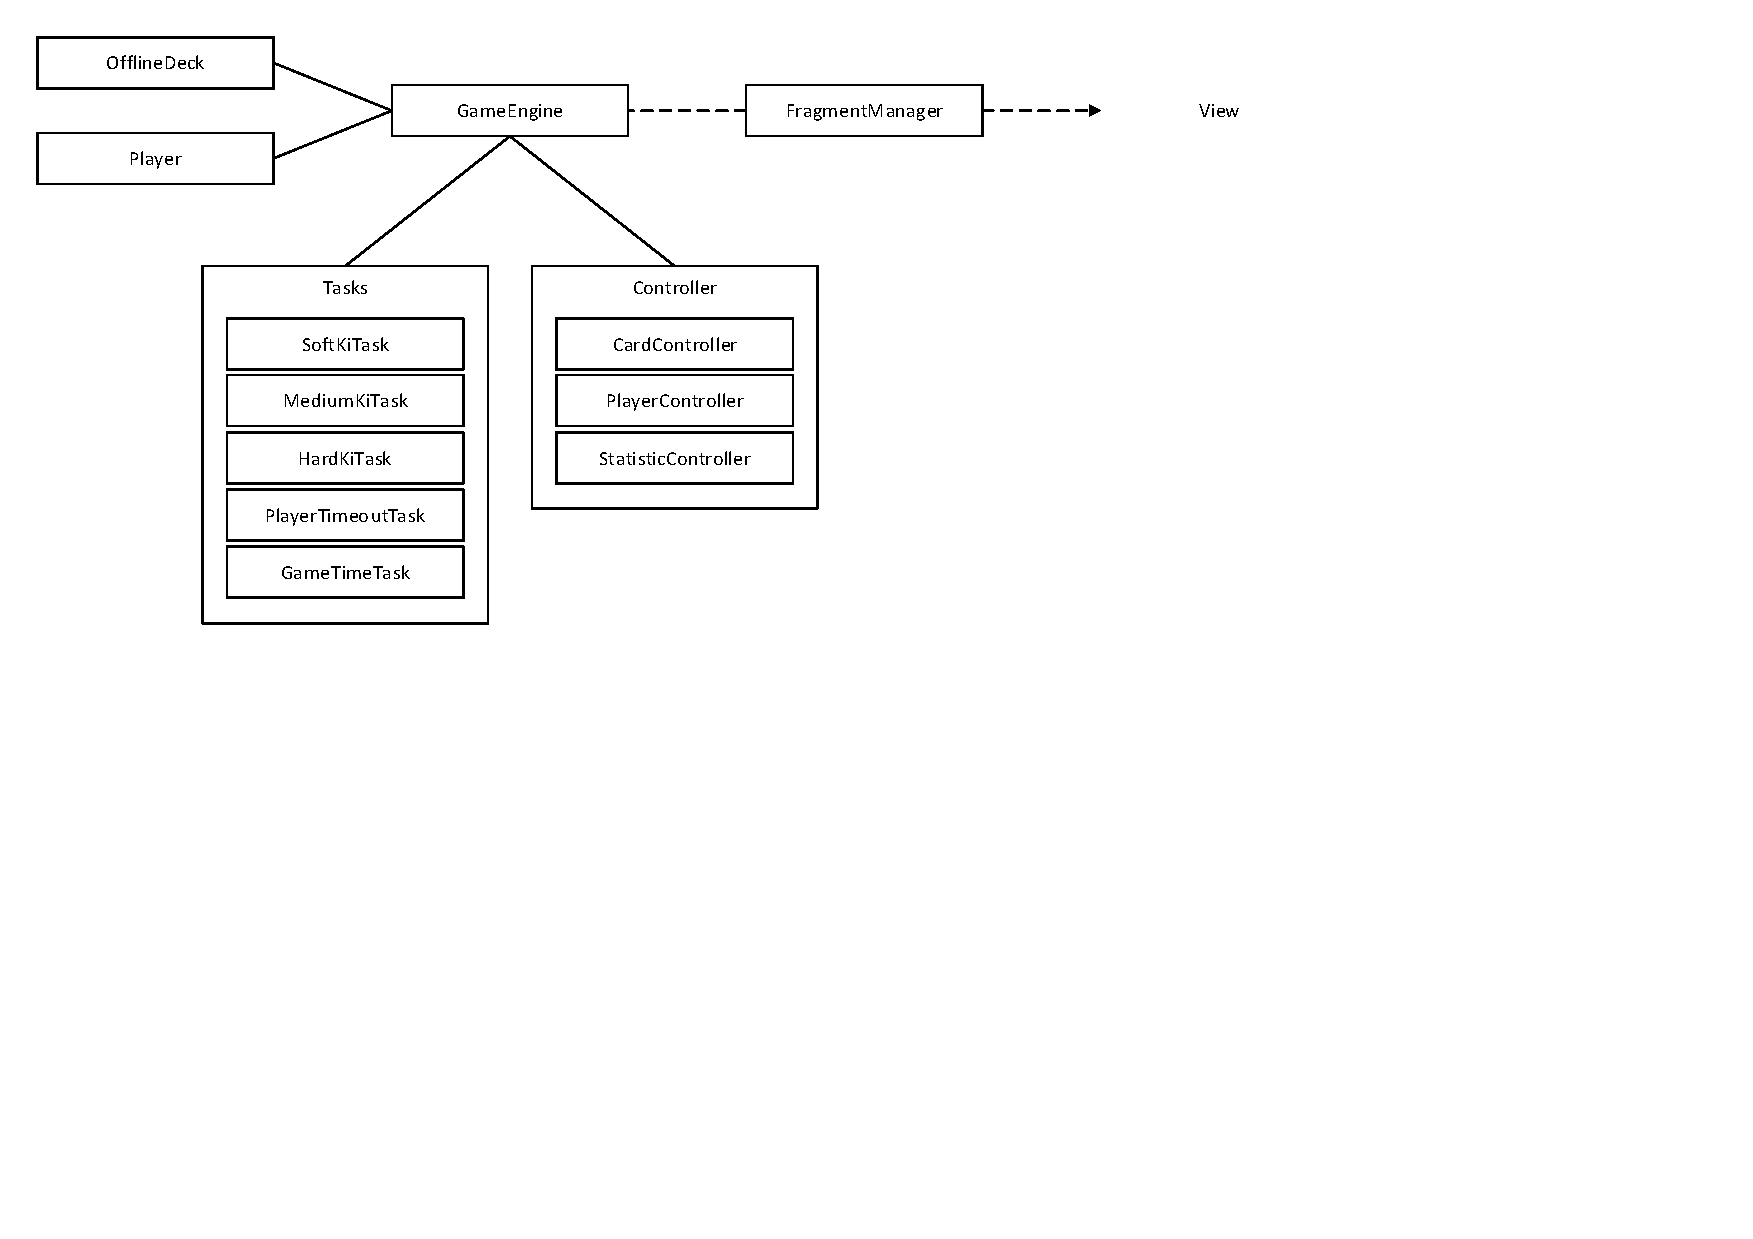
\includegraphics[trim=0 280 220 0,width=\textwidth]{../img/ArchitekturGameengine.pdf}
    \caption{Aufbau der GameEngine Klasse}
    \label{fig:architecture_gameengine}
\end{figure}

Im Folgenden werden die Komponenten aus Abbildung \ref{fig:architecture_gameengine} kurz erläutert:

\begin{itemize}
\item{\textbf{Player}\quad 
Jeder Spieler wird in einem Player-Objekt gespeichert.
}
\item{\textbf{OfflineDeck}\quad
Das Kartendeck welches im aktuellen Spiel verwendet wird.
}
\item{\textbf{Tasks}\quad
Hierbei werden verschiedene Typen verwendet, welche von der Klasse \emph{AsyncTask} erben:
	\begin{itemize}
	\item{\textbf{SoftKiTask}\quad
	Einfacher Computergegner, der einen Spielzug ausführt.
	}
	\item{\textbf{MediumKiTask}\quad
	Mittlerer Computergegner, der einen Spielzug ausführt.	
	}
	\item{\textbf{HardKiTask}\quad
	Schwerer Computergegner, der einen Spielzug ausführt.
	}
	\item{\textbf{PlayerTimeoutTask}\quad
	Zählt die Zeit herunter, die ein Spieler pro Zug zur Verfügung hat. Falls die Zeit abgelaufen ist wird ein beliebiges Attribut gewählt.
	}
	\item{\textbf{GameTimeTask}\quad
	Zählt die Zeit herunter, die für ein Spiel festgelegt wurde.
	}
	\end{itemize}
\item{\textbf{Controller}\quad
Hierbei wurden verschieden Typen verwendet:
	\begin{itemize}
	\item{\textbf{CardController}\quad
	Regelt die Kartenverteilung zu jedem Zeitpunkt des Spiels. 
	}
	\item{\textbf{PlayerController}\quad
	Regelt die Punkteverteilung und ist für die Festlegung des Gewinners zuständig.
	}
	\item{\textbf{StatisticController}\quad
	Regelt die Statistiken und schreibt diese in die \emph{Shared Preferences}
	}
	\end{itemize}
}
\item{\textbf{FragmentManager}\quad
Ist dafür zuständig dass nach jeder Runde eine neue Karte angezeigt wird.
}
}
\end{itemize}

Das komplette Spiel beruht auf dem \emph{Listenerkonzept}, d.h. es gibt keine Schleife die dauerhaft nach Ereignissen sucht. Somit ist wird z.B. nach jedem Spielzug oder nachdem ein Dialogfenster geschlossen wurde eine Nachricht an die \emph{GameEnginge} gesendet, die dann weitere Funktionen aufruft.


\section{Views}
Die Views der in Abschnitt \ref{sec:activities_in_fancyquartett} erläuterten Activities sind allesamt als Fragment implementiert. Jede Activity enthält also mindestens ein Fragment, in welchem das eigentliche Layout ausgerollt wird. Rückwirkend war das für dieses Projekt wohl ein unnötiger Zusatzaufwand, da das Game aktuell nur für Smartphones optimiert ist. Der Vorteil alles mit dem Fragment-Konzept zu implementieren hätte sich unter anderem erst ausgewirkt, wenn das Game auch für andere Formfaktoren wie z.B. Tablets hätte optimiert werden müssen, denn dann hätte das Layout mithilfe der Fragments sehr leicht angepasst werden können. Obwohl dies keine direkte Anforderung war wollten wir uns diese Option trotzdem offen halten.




